
\documentclass{article}
\usepackage[utf8]{inputenc}
\usepackage{tikz}
\usepackage{amsmath}

\begin{document}

\section*{Number Line for Arithmetic Operations}

\subsection*{1. 9 - 5}

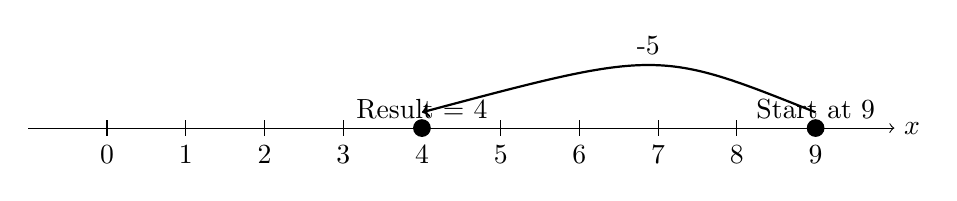
\begin{tikzpicture}
  \draw[->] (-1,0) -- (10,0) node[right] {$x$};
  \foreach \x in {0,1,...,9}
    \draw (\x,0.1) -- (\x,-0.1) node[below] {\x};
  \filldraw (9,0) circle (3pt) node[above] {Start at 9};
  \draw[->,thick] (9,0.2) .. controls (7,1) .. (4,0.2) node[midway,above] {-5};
  \filldraw (4,0) circle (3pt) node[above] {Result = 4};
\end{tikzpicture}

\vspace{1cm}

\subsection*{2. 4 + 3}

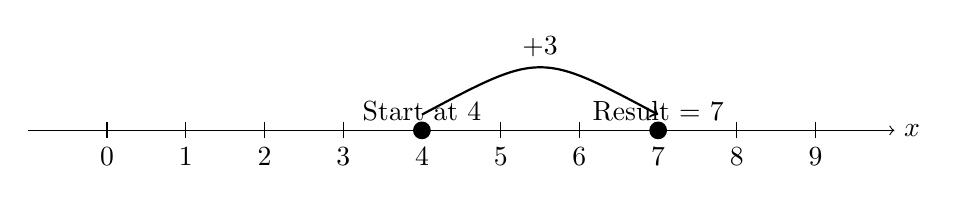
\begin{tikzpicture}
  \draw[->] (-1,0) -- (10,0) node[right] {$x$};
  \foreach \x in {0,1,...,9}
    \draw (\x,0.1) -- (\x,-0.1) node[below] {\x};
  \filldraw (4,0) circle (3pt) node[above] {Start at 4};
  \draw[->,thick] (4,0.2) .. controls (5.5,1) .. (7,0.2) node[midway,above] {+3};
  \filldraw (7,0) circle (3pt) node[above] {Result = 7};
\end{tikzpicture}

\vspace{1cm}

\subsection*{3. -2 + 7}

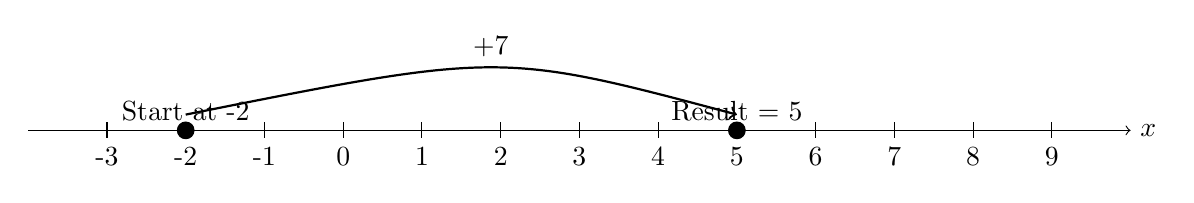
\begin{tikzpicture}
  \draw[->] (-4,0) -- (10,0) node[right] {$x$};
  \foreach \x in {-3,-2,-1,0,1,2,...,9}
    \draw (\x,0.1) -- (\x,-0.1) node[below] {\x};
  \filldraw (-2,0) circle (3pt) node[above] {Start at -2};
  \draw[->,thick] (-2,0.2) .. controls (2,1) .. (5,0.2) node[midway,above] {+7};
  \filldraw (5,0) circle (3pt) node[above] {Result = 5};
\end{tikzpicture}

\vspace{1cm}

\section*{LCM of 18, 36, and 45 (Table Method)}

\begin{tabular}{|c|c|c|c|}
\hline
\textbf{Step} & 18 & 36 & 45 \\
\hline
Divide by 2 & 9 & 18 & 45 \\
\hline
Divide by 2 & 9 & 9 & 45 \\
\hline
Divide by 3 & 3 & 3 & 15 \\
\hline
Divide by 3 & 1 & 1 & 5 \\
\hline
Divide by 5 & 1 & 1 & 1 \\
\hline
\end{tabular}

\vspace{0.5cm}

\noindent
\textbf{LCM} = \( 2 \times 2 \times 3 \times 3 \times 5 = 180 \)

\vspace{1cm}

\section*{HCF of 36 and 45 (Table Method)}

\begin{tabular}{|c|c|c|}
\hline
\textbf{Prime Factor} & 36 & 45 \\
\hline
2 & $2^2$ & -- \\
\hline
3 & $3^2$ & $3^2$ \\
\hline
5 & -- & $5^1$ \\
\hline
\end{tabular}

\vspace{0.5cm}

\noindent
Common factors: \( 3^2 \)

\noindent
\textbf{HCF} = \( 3^2 = 9 \)

\end{document}
